
\section{Geister}

Um das Rechengebiet $\Omega$, in dessen Inneren die \textsc{Maxwells}chen Gleichungen zu lösen sind, räumlich zu diskretisieren, wird es in endlich viele Teilgebiete unterteilt. Eine der gebräuchlichsten Gitterformen ist die kartesische bei der das Rechengebiet in einzelne Quader zerlegt wird. Bei Indizierung der Kanten, Flächen und Volumen mit dem kanonischen Nummerierungsschema, gibt es zu jedem Punkt drei Kanten, drei Flächen und ein Volumen. Dabei werden auch Kanten außerhalb des Rechengebiets durchnummeriert die für die spätere Lösung nicht benötigt werden. Diese nennt man Geisterkanten und findet sie immer am positiven Ende des Bereichs. Anschaulich erkennen kann man dies in Abbildung \ref{fig:geister}, der schwarze Quader ist das Rechengebiet $\Omega$, in Blau sind die Geisterkanten eingezeichnet.

\begin{figure}[thbp]
	\centering
	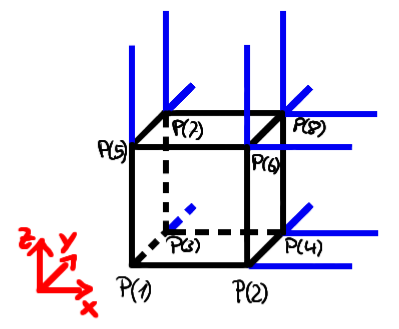
\includegraphics[width=.5\textwidth]{data/Geister}
	\caption{Einfaches Gitter mit Geisterkanten in Blau}
	\label{fig:geister}
\end{figure}

Bei einem Gitter der Größe $ N_x \times N_y \times N_z$ erhält man genau $N_x N_y + N_y N_z + N_x N_z$ Geisterkanten und -flächen, die Anzahl an Geistervolumen beträgt $N_x N_z + N_x (N_y - 1) +(N_y - 1)(N_z - 1)$. Setzt man die Geisterkanten bzw -flächen ins Verhältnis zu allen Kanten bzw Flächen so skalieren sie zu 

\begin{equation*}
	\frac{\mathrm{Geisterkanten}}{\mathrm{Alle \: Kanten}} = \frac{1}{3}(\frac{1}{N_x} + \frac{1}{N_y} + \frac{1}{N_z})
\end{equation*}

und alle Geistervolumen im Vergleich zu allen Volumen 

\begin{equation*}
		\frac{\mathrm{Geistervolumen}}{\mathrm{Alle \: Volumen}} = \frac{N_x N_y + N_y N_z + N_x N_z - N_x - N_y - N_z + 1}{N_x N_y N_z}.
\end{equation*}

Da die Geisterkanten außerhalb des Rechengebiets liegen ist es nicht nötig für diese auch das Integral zu berechnen. Für die Skizze in Abbildung \ref{fig:geister} ist es also sinnvoll nur für die schwarzen Kanten und nicht die blauen das Integral zu berechnen. Wendet man die weiter oben erwähnte Matlab-Implementierung des Gradientenoperators auf das Beispiel an so erhält man in der ersten Zeile die Potential-Differenz zwischen den Punkten $P(1)$ und $P(2)$. Zeile 2 hingegen ergibt die Potential-Differenz zwischen den Punkten $P(2)$ und $P(3)$. Diese Berechnung ist nicht sinnvoll und kommt daher, dass die eigentlich von $P(2)$ ausgehende Kante in $x$-Richtung eine Geisterkante ist. Also sollten Zeile 2 und auch alle anderen die eine Potential-Differenz diagonal durch den Quader berechnen auf null gesetzt werden.


